% !TEX program = xelatex
% AY2021 材料力学 解答例（同志社 生命医科学 医工学コース 院試）
% 問題・図は 01_exams/2021/tex を土台に、参考/ の粒度で解答を付した。
\documentclass[11pt,a4paper]{article}
\usepackage{../../00_common/preamble}
\usetikzlibrary{positioning,arrows.meta,calc,patterns,decorations.pathmorphing}

\title{材料力学 AY2021 解答例}
\author{}
\date{}

\begin{document}
\maketitle

\noindent\textbf{符号規約}：軸力・応力・伸びは引張りを正，圧縮を負とする．
組合せ棒では上向き変位を正にとり，下面を固定（変位 0），上部の剛体円板は床に固定されず
軸方向に平行移動できるものとする（図のモデル化）．曲げ・ねじりは大きさを求め，向きは本文で述べる．

%====================================================================
\section*{〔I〕}

丸棒 1（直径 $d$, 縦弾性係数 $E$, 上部 A--B, 長さ $L/2$）, 丸棒 2（直径 $d$, 縦弾性係数 $3E$,
下部 B--C, 長さ $L/2$）, 円管 3（内径 $4d$, 外径 $6d$, 縦弾性係数 $2E$, 全長 $L$）からなる組合せ棒．
下面は固定され，上面は剛体円板で連結（丸棒 1 と円管 3 の上端を結ぶ）されており，
2 本の丸棒の接合点 B に下向きの外力 $P$ が作用する．

\begin{center}
% 縦断面図（問題図を簡略再現）
\begin{tikzpicture}[>=Latex,scale=0.95]
  \draw[thick] (-2.0,0) -- (2.0,0);
  \foreach \x in {-1.9,-1.6,...,1.95} {\draw (\x,0) -- (\x-0.25,-0.25);}
  \draw[line width=2pt] (-2.0,5.0) -- (2.0,5.0);
  \fill[gray!20] (-1.5,0) rectangle (-1.2,5.0);
  \fill[gray!20] (1.2,0) rectangle (1.5,5.0);
  \draw (-1.5,0) rectangle (-1.2,5.0); \draw (1.2,0) rectangle (1.5,5.0);
  \draw (-0.3,2.5) rectangle (0.3,5.0);
  \fill[gray!35] (-0.3,0) rectangle (0.3,2.5); \draw (-0.3,0) rectangle (0.3,2.5);
  \node[left] at (-0.3,4.6) {A}; \node[left] at (-0.3,2.6) {B}; \node[right] at (0.3,0.3) {C};
  \fill (0,2.5) circle (1.6pt);
  \draw[->,very thick] (0,2.5) -- (0,1.4) node[midway,right]{$P$};
  \node[right] at (0.35,3.9) {\footnotesize 丸棒 1};
  \node[right] at (0.35,1.4) {\footnotesize 丸棒 2};
  \node[right] at (1.55,4.3) {\footnotesize 円管 3};
  \draw[<->] (-1.85,0) -- (-1.85,5.0) node[midway,fill=white]{$L$};
  \draw[<->] (-0.8,0) -- (-0.8,2.5) node[midway,fill=white,font=\scriptsize]{$L/2$};
  \draw[->,line width=1pt] (2.2,4.7) arc (70:-20:1.4) node[midway,right]{$T$};
\end{tikzpicture}

\vspace{1mm}
図1
\end{center}

\begin{enumerate}[label=(\arabic*)]
  \item 丸棒 1, 2 および円管 3 に生じる内力 $N_1$, $N_2$, $N_3$ を求めよ.
  \item 丸棒 1, 2 および円管 3 に生じる応力 $\sigma_1$, $\sigma_2$, $\sigma_3$ を求めよ.
  \item 丸棒 1, 2 および円管 3 の伸び $\lambda_1$, $\lambda_2$, $\lambda_3$ を求めよ.
  \item 外力 $P$ に加え, 上部の剛体板に中心軸まわりのトルク $T$ を負荷したときのねじれ角 $\Psi$ を求めよ.
        横弾性係数はすべて $G$ とする.
\end{enumerate}

\subsection*{解答}

まず断面積を求める．丸棒 1, 2 はともに直径 $d$ なので
\[
  A_{\text{r}}=\frac{\pi d^2}{4}.
\]
円管 3 は外径 $6d$（外半径 $3d$），内径 $4d$（内半径 $2d$）なので
\[
  A_3=\pi\big[(3d)^2-(2d)^2\big]=\pi(9-4)d^2=5\pi d^2 .
\]

\medskip
\noindent\textbf{(1)}\quad これは 1 次の不静定問題である．上向きを正として，上部剛体板の変位を $u_T$，
接合点 B の変位を $u_B$ とおく（下面は固定で変位 0）．各部材の内力（引張り正）は伸び量に比例し
\[
  N_1=\frac{E\,A_{\text{r}}}{L/2}\,(u_T-u_B),\quad
  N_2=\frac{3E\,A_{\text{r}}}{L/2}\,(u_B-0),\quad
  N_3=\frac{2E\,A_3}{L}\,(u_T-0).
\]
釣合い式は，節点 B（上の丸棒 1 が引く力 $N_1$，下の丸棒 2 が引く力 $N_2$，外力 $-P$）と，
上部剛体板（丸棒 1・円管 3 が下向きに引く $N_1,N_3$）について
\[
  N_1-N_2-P=0,\qquad -N_1-N_3=0 .
\]
$A_3=20A_{\text{r}}$ を用いてこれらを解くと
\[
  \ans{\;N_1=\frac{20}{83}P\ (\text{引張り}),\quad
        N_2=-\frac{63}{83}P\ (\text{圧縮}),\quad
        N_3=-\frac{20}{83}P\ (\text{圧縮})\;}
\]
検算：$N_1-N_2=\dfrac{20}{83}P+\dfrac{63}{83}P=P$（節点 B の釣合い），
$N_1+N_3=0$（上板の釣合い）をともに満たす ✓．

\medskip
\noindent\textbf{(2)}\quad 応力は内力を断面積で除して
\[
  \sigma_1=\frac{N_1}{A_{\text{r}}}=\frac{(20/83)P}{\pi d^2/4}=\frac{80P}{83\pi d^2},\quad
  \sigma_2=\frac{N_2}{A_{\text{r}}}=-\frac{252P}{83\pi d^2},\quad
  \sigma_3=\frac{N_3}{A_3}=\frac{-(20/83)P}{5\pi d^2}=-\frac{4P}{83\pi d^2}.
\]
\[
  \ans{\;\sigma_1=\frac{80P}{83\pi d^2},\quad
        \sigma_2=-\frac{252P}{83\pi d^2},\quad
        \sigma_3=-\frac{4P}{83\pi d^2}\;}
\]

\medskip
\noindent\textbf{(3)}\quad 各部材の伸びは $\lambda=\dfrac{N\ell}{EA}$ より
\[
  \lambda_1=\frac{N_1(L/2)}{E\,A_{\text{r}}}=\frac{40PL}{83E\pi d^2},\quad
  \lambda_2=\frac{N_2(L/2)}{3E\,A_{\text{r}}}=-\frac{42PL}{83E\pi d^2},\quad
  \lambda_3=\frac{N_3 L}{2E\,A_3}=-\frac{2PL}{83E\pi d^2}.
\]
\[
  \ans{\;\lambda_1=\frac{40PL}{83E\pi d^2},\quad
        \lambda_2=-\frac{42PL}{83E\pi d^2},\quad
        \lambda_3=-\frac{2PL}{83E\pi d^2}\;}
\]
検算：変位の適合条件 $u_T=u_B+\lambda_1$，$u_B=\lambda_2$，$u_T=\lambda_3$ より
$\lambda_3=\lambda_1+\lambda_2$ が成り立つ．実際
$\lambda_1+\lambda_2=\dfrac{(40-42)PL}{83E\pi d^2}=-\dfrac{2PL}{83E\pi d^2}=\lambda_3$ ✓．

\medskip
\noindent\textbf{(4)}\quad ねじりでは，丸棒 1 と丸棒 2 は接合点 B を介して直列，円管 3 は両者と並列に
上部剛体板と下面を結ぶ．断面二次極モーメントは
\[
  J_{\text{r}}=\frac{\pi d^4}{32}\ (\text{丸棒}),\qquad
  J_3=\frac{\pi\big[(6d)^4-(4d)^4\big]}{32}=\frac{\pi(1296-256)d^4}{32}=\frac{1040\pi d^4}{32}.
\]
内棒（丸棒 1＋丸棒 2）が分担するトルクを $T_{\text{r}}$ とすると，直列なので
\[
  \Psi=T_{\text{r}}\!\left(\frac{L/2}{GJ_{\text{r}}}+\frac{L/2}{GJ_{\text{r}}}\right)=\frac{T_{\text{r}}L}{GJ_{\text{r}}}
  \;\Longrightarrow\; T_{\text{r}}=\frac{GJ_{\text{r}}}{L}\Psi .
\]
円管 3 が分担するトルクは $T_3=\dfrac{GJ_3}{L}\Psi$．並列なので $T=T_{\text{r}}+T_3$ より
\[
  T=\frac{G\Psi}{L}\big(J_{\text{r}}+J_3\big)
   =\frac{G\Psi}{L}\cdot\frac{(1+1040)\pi d^4}{32}
   =\frac{1041\pi G d^4}{32L}\,\Psi .
\]
よって
\[
  \ans{\;\Psi=\frac{32\,TL}{1041\,\pi G d^4}\;}
\]
検算：剛性は和をとるので，仮に円管 3 が無い場合は $\Psi=\dfrac{32TL}{\pi Gd^4}$ となり，
円管 3 を加えると分母が $1\to 1041$ 倍に増え $\Psi$ が小さくなる．並列で剛性が増す描像と整合する ✓．

%====================================================================
\clearpage
\section*{〔II〕}

直径 $d$, 長さ $L$ の円形断面はり（固定端 A, 自由端 B）の先端 B に，はり軸と直交する向きに
長さ $L$ の剛体棒が取り付けられ，その先端に鉛直下向きの外力 $F$ が負荷される．
縦弾性係数 $E$, 横弾性係数 $G$ とする．点 Q は $(x=L-a,\ y=0,\ z=d/2)$（上面）にある．

\begin{center}
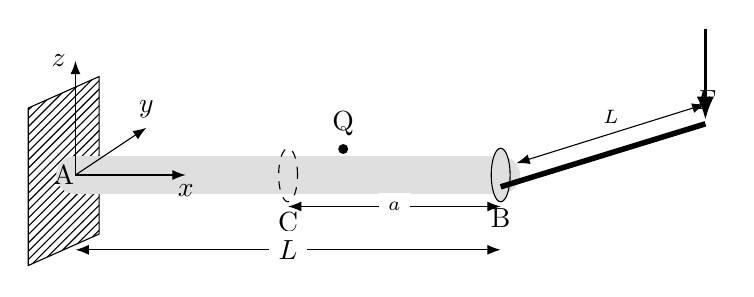
\begin{tikzpicture}[>=Latex]
  \fill[pattern=north east lines] (0.0,-0.6) -- (0.0,1.4) -- (0.9,1.8) -- (0.9,-0.2) -- cycle;
  \draw (0.0,-0.6) -- (0.0,1.4) -- (0.9,1.8) -- (0.9,-0.2) -- cycle;
  \draw[line width=14pt,gray!25,line cap=round] (0.6,0.55) -- (6.0,0.55);
  \draw[fill=gray!25] (6.0,0.55) ellipse (0.12 and 0.34);
  \draw[line width=2pt] (6.0,0.4) -- (8.6,1.2);
  \draw[->,very thick] (8.6,2.4) -- (8.6,1.25) node[above]{$F$};
  \draw[->] (0.6,0.55) -- (0.6,2.0) node[left]{$z$};
  \draw[->] (0.6,0.55) -- (1.5,1.15) node[above]{$y$};
  \draw[->] (0.6,0.55) -- (2.0,0.55) node[below]{$x$};
  \node at (0.45,0.55) {A}; \node[below] at (6.0,0.25) {B};
  \draw[dashed] (3.3,0.55) ellipse (0.12 and 0.34);
  \node at (3.3,-0.05) {C};
  \fill (4.0,0.88) circle (1.8pt); \node[above] at (4.0,0.92) {Q};
  \draw[<->] (0.6,-0.4) -- (6.0,-0.4) node[midway,fill=white]{$L$};
  \draw[<->] (3.3,0.15) -- (6.0,0.15) node[midway,fill=white,font=\scriptsize]{$a$};
  \draw[<->] (6.2,0.7) -- (8.6,1.45) node[midway,above,font=\scriptsize]{$L$};
\end{tikzpicture}

\vspace{1mm}
図2
\end{center}

\begin{enumerate}[label=(\arabic*)]
  \item 固定端 A の支持力, 支持モーメント, 支持トルクを求めよ.
  \item せん断力図（SFD）および曲げモーメント図（BMD）を求めよ.
  \item 点 Q の $x$ 方向応力 $\sigma_x$, 円周方向応力 $\sigma_y$, せん断応力 $\tau_{xy}$ を求めよ.
  \item 点 Q のモールの応力円を描き, 最大主応力を求めよ.
\end{enumerate}

\subsection*{解答}

剛体棒ははり軸（$x$）に直交する $y$ 方向に長さ $L$ で取り付き，その先端（位置 $x=L,\ y=L$）に
鉛直下向き（$-z$）の力 $F$ が作用する．この力を B 点（$x=L,\ y=0$）に移すと，
力 $F$（下向き）と，$y$ 方向の腕 $L$ による $x$ 軸まわりのトルク $T=FL$ が生じる．

\medskip
\noindent\textbf{(1)}\quad はり全体のつり合いより固定端 A の反力を求める．
鉛直方向のつり合いから支持力は
\[
  R_A=F\quad(\text{上向き}).
\]
力 $F$ は固定端から軸方向に $L$（B 点の位置）離れた点に作用するので，曲げの支持モーメントは
\[
  M_A=F\cdot L=FL .
\]
さらに $y$ 方向の腕 $L$ による軸まわりのトルクが伝わるので，支持トルクは
\[
  T_A=F\cdot L=FL .
\]
\[
  \ans{\;R_A=F,\qquad M_A=FL\ (\text{曲げ}),\qquad T_A=FL\ (\text{ねじり})\;}
\]
検算：荷重系は鉛直力 $F$ ただ 1 つなので支持力は $F$，その作用線が固定端から軸方向 $L$・
$y$ 方向 $L$ 離れることから曲げ・ねじりともに $FL$ となり，モーメントのつり合いと整合する ✓．

\medskip
\noindent\textbf{(2)}\quad 横荷重 $F$ は B 点（$x=L$）に集中して作用する．区間 $0\le x\le L$ で断面右側の
つり合いをとると，せん断力は一定，曲げモーメントは固定端で最大の線形分布となる：
\[
  \ans{\;Q(x)=F\ (\text{一定}),\qquad M(x)=F(L-x)\quad(0\le x\le L)\;}
\]
すなわち $M(0)=FL$（固定端 A），$M(L)=0$（自由端 B）．また軸まわりのトルクは全長で一定
$T(x)=FL$ である．

\begin{center}
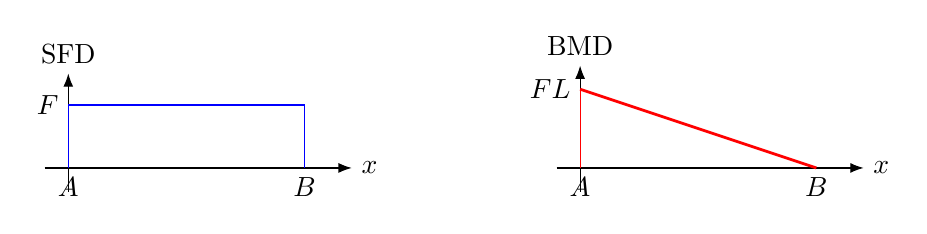
\begin{tikzpicture}[>=Latex,scale=1.0]
  \def\L{3.0}
  \begin{scope}
    \draw[->] (-0.3,0) -- (\L+0.6,0) node[right]{$x$};
    \draw[->] (0,-0.3) -- (0,1.2) node[above]{SFD};
    \draw[line width=1pt,blue] (0,0.8) -- (\L,0.8);
    \draw[blue] (0,0)--(0,0.8); \draw[blue] (\L,0)--(\L,0.8);
    \node[left] at (0,0.8) {$F$};
    \node[below] at (0,0) {$A$}; \node[below] at (\L,0) {$B$};
  \end{scope}
  \begin{scope}[xshift=6.5cm]
    \draw[->] (-0.3,0) -- (\L+0.6,0) node[right]{$x$};
    \draw[->] (0,-0.3) -- (0,1.3) node[above]{BMD};
    \draw[line width=1pt,red] (0,1.0) -- (\L,0);
    \draw[red] (0,0)--(0,1.0);
    \node[left] at (0,1.0) {$FL$};
    \node[below] at (0,0) {$A$}; \node[below] at (\L,0) {$B$};
  \end{scope}
\end{tikzpicture}
\end{center}

\medskip
\noindent\textbf{(3)}\quad 点 Q（$x=L-a$, 上面 $z=d/2$）での応力を求める．円形断面の諸量は
\[
  I=\frac{\pi d^4}{64},\qquad J=\frac{\pi d^4}{32}.
\]
点 Q の断面の曲げモーメントは $M(L-a)=F\big(L-(L-a)\big)=Fa$．上面（$z=d/2$）は引張り側なので
\[
  \sigma_x=\frac{M(L-a)\,(d/2)}{I}=\frac{Fa\,(d/2)}{\pi d^4/64}=\frac{32Fa}{\pi d^3}.
\]
円周（$y$）方向には荷重がなく，はり表面は自由なので
\[
  \sigma_y=0 .
\]
せん断応力はねじり $T=FL$ による表面せん断が寄与する（曲げによる横せん断応力は上面の最外縁で 0）．
表面（半径 $d/2$）では
\[
  \tau_{xy}=\frac{T\,(d/2)}{J}=\frac{FL\,(d/2)}{\pi d^4/32}=\frac{16FL}{\pi d^3}.
\]
\[
  \ans{\;\sigma_x=\frac{32Fa}{\pi d^3},\qquad \sigma_y=0,\qquad \tau_{xy}=\frac{16FL}{\pi d^3}\;}
\]

\medskip
\noindent\textbf{(4)}\quad $\sigma_x=\dfrac{32Fa}{\pi d^3}$, $\sigma_y=0$, $\tau_{xy}=\dfrac{16FL}{\pi d^3}$
の平面応力状態である．モールの応力円は，中心
\[
  c=\frac{\sigma_x+\sigma_y}{2}=\frac{\sigma_x}{2}=\frac{16Fa}{\pi d^3},
\]
半径
\[
  r=\sqrt{\left(\frac{\sigma_x-\sigma_y}{2}\right)^2+\tau_{xy}^2}
   =\sqrt{\left(\frac{16Fa}{\pi d^3}\right)^2+\left(\frac{16FL}{\pi d^3}\right)^2}
   =\frac{16F}{\pi d^3}\sqrt{a^2+L^2}
\]
の円である．

\begin{center}
\begin{tikzpicture}[>=Latex,scale=1.0]
  \def\c{2.2}\def\r{1.5}
  \draw[->] (-0.4,0) -- (5.0,0) node[right]{$\sigma$};
  \draw[->] (0,-2.0) -- (0,2.0) node[above]{$\tau$};
  \draw[line width=1pt,blue] (\c,0) circle (\r);
  \fill (\c,0) circle (1.2pt); \node[below right] at (\c,0) {\scriptsize $c$};
  \fill (\c+\r,0) circle (1.2pt); \node[below] at (\c+\r,-0.05) {\scriptsize $\sigma_{\max}$};
  \fill (\c-\r,0) circle (1.2pt); \node[below] at (\c-\r,-0.05) {\scriptsize $\sigma_{\min}$};
  % 応力点 (σx, -τ) と (σy=0, +τ)
  \fill (\c+0.6,-0.95) circle (1.2pt); \node[right] at (\c+0.6,-0.95) {\scriptsize $(\sigma_x,-\tau_{xy})$};
  \fill (\c-0.6,0.95) circle (1.2pt); \node[left] at (\c-0.6,0.95) {\scriptsize $(\sigma_y,\tau_{xy})$};
  \draw[dashed] (\c-0.6,0.95) -- (\c+0.6,-0.95);
  \node[above] at (\c,\r) {\scriptsize 半径 $r$};
\end{tikzpicture}
\end{center}

主応力は $\sigma=c\pm r$ であるから
\[
  \ans{\;\sigma_{\max}=\frac{16F}{\pi d^3}\Big(a+\sqrt{a^2+L^2}\Big),\qquad
        \sigma_{\min}=\frac{16F}{\pi d^3}\Big(a-\sqrt{a^2+L^2}\Big)\;}
\]
検算：$\sigma_{\max}+\sigma_{\min}=2c=\dfrac{32Fa}{\pi d^3}=\sigma_x+\sigma_y$（応力の不変量・トレース一致），
$\sigma_{\max}\sigma_{\min}=c^2-r^2=-\tau_{xy}^2=\sigma_x\sigma_y-\tau_{xy}^2$（行列式一致）であり，
不変量が保存している ✓．

\end{document}
